\documentclass[conference]{IEEEtran}
% *** GRAPHICS RELATED PACKAGES ***
%
%\ifCLASSINFOpdf

%\else

%\fi

\usepackage{amssymb}
\usepackage{multirow}
\usepackage{rotating}
\usepackage{amsmath}
\usepackage{float}
\usepackage{gensymb}
\usepackage{hyperref}
\usepackage[colorinlistoftodos]{todonotes}
\usepackage[labelfont=scriptsize]{caption}
\renewcommand{\thefigure}{\arabic{figure}}
\renewcommand{\thetable}{\arabic{table}}

%\usepackage[table,xcdraw]{xcolor}
%\usepackage{graphicx}
\usepackage[utf8]{inputenc}
%\usepackage[english]{babel}
\usepackage[backend=biber,style=ieee,sorting=none]{biblatex}
\addbibresource{reference.bib}

\begin{document}

\title{Applied Machine Learning Project 4 \\ Prediction of real estate property prices in Montr\'eal}

\author{\IEEEauthorblockN{Nissan Pow}
\IEEEauthorblockA{McGill University\\
nissan.pow@mail.mcgill.ca}
\and
\IEEEauthorblockN{Emil Janulewicz}
\IEEEauthorblockA{McGill University\\
emil.janulewicz@mail.mcgill.ca}
\and
\IEEEauthorblockN{Liu (Dave) Liu}
\IEEEauthorblockA{McGill University\\
liu.liu2@mail.mcgill.ca}}

% make the title area
\maketitle

% As a general rule, do not put math, special symbols or citations
% in the abstract
\begin{abstract}
In this machine learning paper, we analyzed the real estate property prices in Montr\'eal. The information on the real estate listings was extracted from Centris.ca and duProprio.com. We predicted both asking and sold prices of real estate properties based on features such as geographical location, living area, and number of rooms, etc. Additional geographical features such as the nearest police station and fire station were extracted from the Montr\'eal Open Data Portal. We used and compared regression methods such as linear regression, Support Vector Regression (SVR), k-Nearest Neighbours (kNN), and Regression Tree/Random Forest Regression. We predicted the asking price with an error of 0.0985 using an ensemble of kNN and Random Forest algorithms. In addition, where applicable, the final price sold was also predicted with an error of 0.023 using the Random Forest Regression. We will present the details of the prediction questions, the analysis of the real estate listings, and the testing and validation results for the different algorithms in this paper. In addition, we will also discuss the significances of our approach and methodology.
\end{abstract}

\IEEEpeerreviewmaketitle

\section{Introduction}
Prices of real estate properties is critically linked with our economy \cite{NBERw13553}. Despite this, we do not have accurate measures of housing prices based on the vast amount of data available. In the Montr\'eal island alone, there are around \textbf{15,000} current listings at Centris.ca, and around \textbf{10,000} historical sales at duProprio.com. This dataset has close to a hundred features/attributes such as geographical location, living area, and number of rooms, etc. These features can be supplemented by sociodemographical data from the Montr\'eal Open Data Portal and Statistics Canada. This rich dataset should be sufficient to establish a regression model to accurately predict the price of real estate properties in Montr\'eal.

A property's appraised value is important in many real estate transactions such as sales, loans, and its marketability. Traditionally, estimates of property prices are often determined by professional appraisers. The disadvantage of this method is that the appraiser is likely to be biased due to vested interest from the lender, mortgage broker, buyer, or seller. Therefore, an automated prediction system can serve as an independent third party source that may be less biased.

For the buyers of real estate properties, an automated price prediction system can be useful to find under/overpriced properties currently on the market. This can be useful for first time buyers with relatively little experience, and suggest purchasing offer strategies for buying properties.

One didactic and heuristic dataset commonly used for regression analysis of housing prices is the Boston suburban housing dataset \cite{RePEc:eee:jeeman:v:5:y:1978:i:1:p:81-102}. Previous analyses have found that the prices of houses in that dataset is most strongly dependent with its size and the geographical location \cite{belkuhwel80, Quinlan93combininginstance-based}. More recently, basic algorithms such as linear regression can achieve 0.113 prediction errors using both intrinsic features of the real estate properties (living area, number of rooms, etc.) and additional geographical features (sociodemographical features such as average income, population density, etc.) \cite{RePEc:jre:issued:v:32:n:2:2010:p:139-160, SpatialDependence}.

In the temporal domain, new machine learning algorithms were implemented by Yann LeCun's group to accurately predict the temporal patterns of housing prices in the Los Angeles area \cite{Caplin08machinelearning}. By taking into account geographical data, they were able to more accurately predict the temporal trends in housing prices using basic regression models (0.153 to 0.101).

In this machine learning paper, we predicted the selling prices of properties using regression methods such as linear regression, Support Vector Regression (SVR), k-Nearest Neighbours (kNN), and Regression Tree/Random Forest Regression. We predicted the asking price with an error of 0.0985 using an ensemble of kNN and Random Forest methods. We will present the details of the analysis, and the testing and validation results for the different algorithms below. In addition, we will also discuss the significances of our approach and methodology.

\section{Prediction Question and Dataset}
The prediction question is to predict the price of real estate properties using intrinsic features from the real estate listings themselves, and additional geographical features from the Montr\'eal Open Data Portal and Statistics Canada. Although the features used for prediction are the same across the entire dataset, the targets to be predicted can have subtle differences depending on the intended usage of the prediction. For example, for the buyers to determine under/overpriced properties currently on the market, the predicted asking price may be the most useful. Since predictions that are significantly above the actual asking price may be underpriced properties, and the predictions that are significantly below the actual asking price may be overpriced properties (Fig. \ref{pred1}). In another scenario, for the sellers to accurately estimate the market value of their properties, the prediction of the final prices sold may be more useful. For this reason, we collected data for current real estate listings from Centris.ca, as well as completed real estate sales in Montr\'eal from duProprio.com.

The price sold is usually close to 0.030 of the asking price for real estate properties in Canada (Realtor.ca and Fig. \ref{askVsold}). We also used the asking price with all features to predict the price sold, and achieved an error of 0.023. This is an additional advantage of our prediction system as buyers can use our predictions to more accurately estimate an appropriate offer price for the listings.\\

\begin{figure}[H]
\centering
\includegraphics[width=0.5\textwidth]{askingVsSold.png}
\caption{\scriptsize The final sold price plotted against the asking price.}
\label{askVsold}
\end{figure}

The dataset has approximately \textbf{25,000} examples (15,000 from Centris.ca and 10,000 from duProprio.com) and \textbf{130} features. Examples of features that accounted for the most variance in the target prices are listed in Table \ref{vaf} of the Results section. The features (around \textbf{70}) from the real estate listings were mainly scraped from central listing websites, Centris.ca and duProprio.com. Some additional important features such as living area, municipal evaluation, and school tax need to be further scraped from individual real estate agencies such as, RE/MAX, Century 21, and Sutton, etc.

Since geographical location can account for some spatial and temporal trends in the prices \cite{Caplin08machinelearning}, we incorporated additional sociodemographical features (around \textbf{60}) based on the Montr\'eal borough where the property is located. The corresponding Montreal borough that a property belongs to was determined by inputting the GPS coordinate of its address to the bounding polygons that define the Montreal boroughs. The bounding polygons were obtained from the Montreal Open Data Portal\footnote{http://donnees.ville.montreal.qc.ca/dataset/polygones-arrondissements} and the sociodemographical features are from the 2006 and 2011 census at Statistics Canada. Examples of the sociodemographical features are the population density, average income, and average family size, etc. for the borough. In addition, we incorporated the geographical distance to the nearest fire station and police station. These datasets were also obtained from the Montreal Open Data Portal\footnote{http://donnees.ville.montreal.qc.ca/dataset/carte-postes-quartier}.

Overall, we found these additional geographical features reduced the prediction error by approximately 0.02 (0.13 to 0.11 across the algorithms). This is comparable to the improvement found for the Boston suburban dataset (0.122 to 0.109) \cite{belkuhwel80}, but weaker than the improvement in the prediction of temporal trends (0.153 to 0.101) \cite{Caplin08machinelearning}. 

\section{Methods}
\subsection{Data pre-processing}
In general, the data parsed from raw HTML files may have mistakes both in the original record or initial processing. Outliers were determined by human inspection of the distribution of values, and subsequently removed/corrected. Fortunately, only a few of the examples had missing values, and these can be excluded from further analysis.

Properties with prices less than \$10,000 were not included in the analysis since they were likely to be errors in original data recording or the retrieval process. In addition, we considered properties over 4 times the interquartile range to be outliers. This resulted in 186 out of 7,385 apartments in Montr\'eal to be outliers (Fig. \ref{outlier}). Human inspection of some of these price outliers concluded that they require additional features to accurately predict. For example, some of these apartments included expensive interior decorations and/or furniture in the listing price.

\begin{figure}[H]
\centering
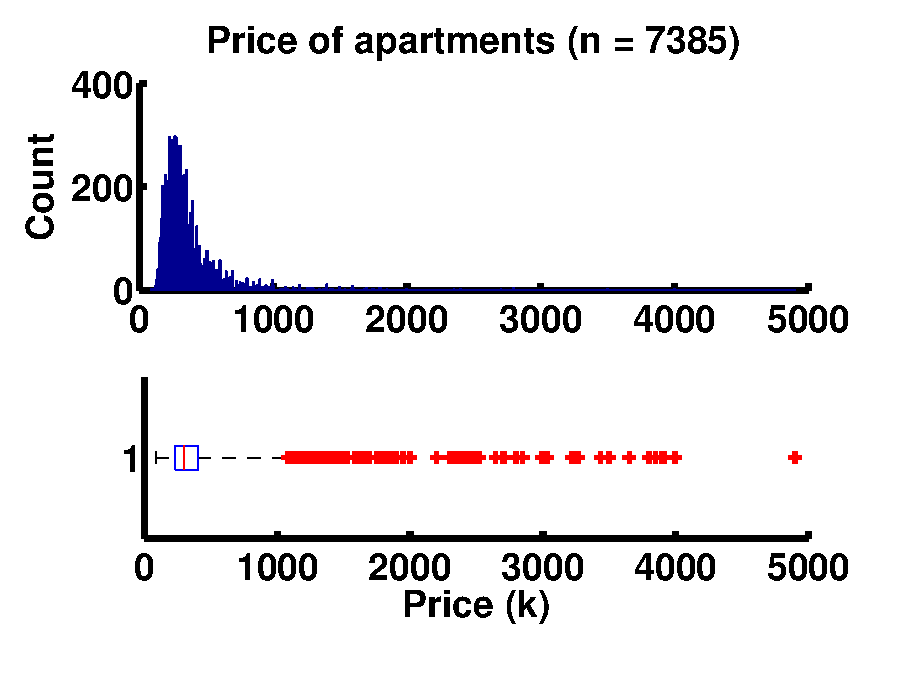
\includegraphics[width=0.5\textwidth]{outlier.eps}
\caption{\scriptsize Distribution of apartment prices in Montr\'eal. Histogram with 500 bins shows a highly skewed distribution of apartment prices. Box-and-whisker plot using whisker length of 4 of interquartile range. The prices that fall outside of the whiskers are consider outliers and are not used in the prediction regression.}
\label{outlier}
\end{figure}

\subsection{Feature design and selection}
The full set of numerical features can be readily used, and gives good prediction error in our results (Table \ref{compar}) that is comparable with previous literature \cite{SpatialDependence,RePEc:jre:issued:v:32:n:2:2010:p:139-160,Caplin08machinelearning}. However, we did attempt some feature engineering as described below.

For the living area of the properties, we used a logarithmic scale since differences in size of smaller properties have a bigger influence on price than differences in size of larger properties \cite{SpatialDependence}. However, this did not improve our prediction error.

To account for temporal factors in the price, we represented the year as a categorical variable as described in \cite{NBERw13553}. We also found that by incorporating the value of the Montreal Housing Price Index (HPI)\footnote{\url{http://homepriceindex.ca/hpi_tool_en.html}} for the month when the listing was sold, we were able to reduce the error by 0.01.

To reduce the dimensionality, we used Principal Component Analysis (PCA) to project the examples onto a lower dimensional space. We selected the orthogonal principal components (PC) that represent the most variance in the data \cite{bishop2006pattern}. PCA can benefit algorithms such as kNN that relies heavily on the distance between examples in the feature space \cite{bishop2006pattern}. However, this did not improve the performance of our kNN algorithm. This is possibly due to that many of the features are noisy compared to the most informative ones (Table. \ref{vaf}). When we used the top 3 features with the highest coefficients from linear regression, we did observe an improvement in kNN performance (see kNN results for more detail), as the magnitude of the coefficients in linear regression are a good proxy for the importance of the feature \cite{Guyon2002}.

Overall, we felt the number of examples in our dataset was sufficient for the training of regression models as the learning curves with one of our top regression model (Random Forest Regression) showed a plateau in prediction error with 90\% of the dataset (Fig. \ref{lr1} and \ref{lr2}).

\begin{figure}[H]
\centering
\includegraphics[width=0.5\textwidth]{perDiff.png}
\caption{\scriptsize Random Forest Regression performance as a function of the amount of data. Results are from 10-fold cross-validation from the subset of data.}
\label{lr1}
\end{figure}

\begin{figure}[H]
\centering
\includegraphics[width=0.5\textwidth]{var.png}
\caption{\scriptsize The variance of the prediction errors in Fig. \ref{lr1}.}
\label{lr2}
\end{figure}

\section{Algorithm Selection, Optimization, and Parameters}
We selected the following algorithms for regression of prices: Linear Regression, Support Vector Regression (SVR), k-Nearest Neighbours (kNN), and Random Forest Regression. The algorithms were implemented using Python's scikit-learn library \cite{scikit-learn}.

\subsection{Linear regression}
To establish baseline performance with a linear classifier, we used Linear Regression to model the price targets, $Y$, as a linear function of the data, $X$ \cite{bishop2006pattern,hastie2009elements}.
\begin{align*}
f_\bold{w}(\bold{X}) &= w_0 + w_1x_1 + ... + w_mx_m\\
&= w_0 + \sum_{j=1:m}w_jx_j
\end{align*}
Where $w_j$ are the weights of the features, $m$ are the number of features and $w_0$ is the weight to the bias term, $x_0=1$.

The weights of the linear model can be found with the least-square solution method, where we find the $\bold{w}$ that minimizes:
\begin{align*}
Err(w) = \sum_{i=1:n}(y_i-\bold{w^Tx_i})^2
\end{align*}
Here $\bold{w}$ and $\bold{x}$ are column vectors of size $m+1$.

Re-writing in matrix notation we have:
\begin{align*}
f_\bold{w}(\bold{X}) &= X\bold{w}\\
Err(\bold{w}) &= (Y-X\bold{w})^T(Y-X\bold{w})
\end{align*}
where $X$ is the $n \times m$ matrix of input data, $Y$ is the $n \times 1$ vector of output data, and $\bold{w}$ is the $m \times 1$ vector of weights.

To minimize the error, take the derivative w.r.t. $\bold{w}$ to get a system of $m$ equations with $m$ unknowns:
\begin{align*}
\partial Err(\bold{w})/\partial \bold{w} = -2X^T(Y-X\bold{w})
\end{align*}
Set the equation to 0 and and solve for $\bold{w}$:
\begin{align*}
X^T(Y-X\bold{w})&=0\\
X^TY&=X^TX\bold{w}\\
\hat{\bold{w}}&=(X^TX)^{-1}X^TY
\end{align*}
where $\hat{\bold{w}}$ denotes the estimated weights from the closed-form solution.

To speed up computation, the weights can be fitted iteratively with a gradient descent approach.

Given an initial weight vector $\bold{w_0}$, for $k=1,2,...,m, \bold{w}_{k+1}=\bold{w}_k-\alpha_k \delta Err(\bold{w}_k)/\delta \bold{w}_k$, and end when $|\bold{w}_{k+1}-\bold{w}_k|< \epsilon$.

Here, parameter $\alpha_k>0$ is the learning rate for iteration $k$.

The performance of linear regression is in Table \ref{compar}.

\subsection{Support Vector Regression (SVR)}
We used the linear SVR and also the polynomial and Gaussian kernels for regression of target prices \cite{Cortes:1995:SN:218919.218929,bishop2006pattern}.\\
The linear SVR estimates a function by maximizing the number of deviations from the actually obtained targets $y_n$ within the normalized margin stripe, $\epsilon$, while keeping the function as flat as possible \cite{Vapnik:1995:NSL:211359}. In other word, the magnitude of the error does not matter as long as they are less than $\epsilon$, and \textit{flatness} in this case means minimize $w$. For a data set of $N$ target prices with $M$ features, there are feature vectors $x_n \in R^M$ where $n=1,...,N$ and the targets $y_n$ corresponding to the price of real estate properties. The SVR algorithm is a convex minimization problem that finds the normal vector $\bold{w}\in R^M$ of the linear function as follows \cite{Smola:2004:TSV:1011935.1011939}:

\begin{align*}
\underset{\bold{w},\gamma}{\operatorname{min}} \left(\frac{1}{2}||\bold{w}||^2 + C \sum\limits_{n=1}^N\gamma_n+\gamma_n^\star\right)
\end{align*}
subject to the constraints for each $n$:
\begin{align*}
y_n - \left( \bold{w}*\bold{x}_n \right) &\leq \epsilon+\gamma_n,\\
\left( \bold{w}*\bold{x}_n \right)-y_n &\leq \epsilon+\gamma_n^\star, \\ \gamma_n,\gamma_n^\star &\geq 0
\end{align*}

Where $\gamma_n, \gamma_n^\star$ are 'slack' variables allowing for errors to cross the margin. The constant $C>0$ determines the trade off between the flatness of the function and the amount up to which deviations larger than $\epsilon$ are tolerated \cite{Bennett92robustlinear}.

The results for the SVR can be found in Fig. \ref{pred1} and Table \ref{compar}.

\subsection{k-Nearest Neighbours (kNN)}
k-Nearest-Neighbour (kNN) is a non-parametric instance based learning method. In this case, training is not required. The first work on kNN was submitted by Fix \& Hodges in 1951 for the United States Air-force \cite{fix1951discriminatory}.

The algorithm begins by storing all the input feature vectors and outputs from our training set. For each unlabeled input feature vector, we find the $k$ nearest neighbors from our training set. The notion of \textit{nearest} uses Euclidean distance in the $m$-dimensional feature space. For two input vectors $\bold{x}$ and $\bold{w}$, their distance is defined by:
$$d(\bold{x,w})=\sqrt{\sum_{i=1}^{m}(x_i-w_i)^2}$$
Once the $k$ nearest neighbors are selected, the predicted value can either be the average of the $k$ neighbouring outputs (uniform weighting), or a weighted sum defined by some function. We will propose a good choice of such a function based on geographic distance between the test point and its neighbours.

In our analysis we use leave-one-out cross-validation. In this case, if we start with $n$ input vectors, each sample is predicted based on the other $n-1$ input vectors. 

Before passing our data through a kNN regressor, we first used a Standard Scaler (scikit-learn) on our input data. This transforms each feature column vector to have zero mean and unit variance. With all features normalized, each feature has a fair weight in estimating the Euclidean distance and there will be no dominating features.

It has been shown in previous studies that there is strong spatial dependency between house values \cite{Caplin08machinelearning,SpatialDependence}. Thus we argue that geographical distance between houses will have a large impact on the predicted value. We use a Gaussian Kernel to weight the output of our neighbors:
 $$e^{-\frac{d^2}{2\sigma^2}}$$
where $d$ is the geographical shortest distance between the two points (in km) and $\sigma$ is a hyper-parameter to be optimized. We note that by making $\sigma$ smaller, we are weighting our prediction more on the nearest neighbours that are also close in a geographic sense. This is very intuitive since houses with similar features that are also close geographically should have similar values. In fact, the same line of reasoning would be used by a broker to estimate the price of a house, i.e. looking at the value of nearby houses with similar features.

\subsection{Random Forest Regression}
The Random Forest Regression (RFR) is an ensemble algorithm that combines multiple Regression Trees (RTs). Each RT is trained using a random subset of the features, and the output is the average of the individual RTs. 

The sum of squared errors for a tree T is:

$ \displaystyle S = \sum_{c \in leaves(T)}\sum_{i \in C}(y_{i}-m_{c})^{2}$ \\
where $\displaystyle m_{c} = \frac{1}{n_{c}}\sum_{i \in C}y_{i}$, the prediction for leaf $c$.

Each split in the RT is performed in order to minimize $S$. The basic RT growing algorithm is as follows:

\begin{enumerate}
\item Begin with a single node containing all points. Calculate $m_{c}$ and $S$
\item If all the points in the node have the same value for all the independent variables, then stop. Otherwise, search over all binary splits of all variables for the one which will reduce $S$ the most. If the largest decrease in
$S$ would be less than some threshold $\delta$, or one of the resulting nodes would
contain less than $q$ points, then stop. Otherwise, take that split, creating two new nodes.
\item In each new node, go back to step 1.
\end{enumerate}

One problem with the basic tree-growing algorithm is early termination. An approach that works better in practice is to fully grow the tree (ie, set $q=1$ and $\delta=0$), then prune the tree using a holdout test set.

\section{Results}

The results below are reported in the order based on how they performed (worst to best, Table. \ref{compar}) The prediction errors reported used 10-fold cross-validation unless otherwise noted. We looked at both the mean absolute percentage difference (Fig. \ref{lr1}) and also its variance (Fig. \ref{lr2}). Presumably, the mean and variance should be correlated, however, decrease of either one indicate an improvement in the performance of our model.

\subsection{Linear regression and SVR}

Linear regression using Lasso (L1) regularization and the SVR had similar performances (Table \ref{compar}). 

\begin{table}[htbp]
\footnotesize
\centering
\caption{\footnotesize Variance Accounted For (VAF) in the target price for different features using the linear regression.}
\begin{tabular}{|c|c|c|c|c|c|}
\hline
Feature & Area & \# Rm & \# Bedroom & \# Bathroom & Pool\\ \hline
VAF & 0.472 & 0.141 & 0.158 & 0.329 & 0.110\\
\hline
\end{tabular}
\label{vaf}
\end{table}
\normalsize

We used the SVR with different kernels to predict the target prices (Fig. \ref{pred1} and Table. \ref{svm}). Interestingly, the linear kernel had the best performance (Table. \ref{svm}).

\begin{figure}[H]
\centering
\includegraphics[width=0.5\textwidth]{predict1.png}
\caption{\scriptsize SVR using features from the listings. Results are from 10-fold cross-validation. Plotting the predicted price vs. the actual price can be useful for the buyers, since the points that are largely above the unity slope line may be properties that are undervalued, and the points that are largely below the unity line may be properties that are overvalued.}
\label{pred1}
\end{figure}

\begin{table}[htbp]
\footnotesize
\centering
\caption{\footnotesize SVM performance with different kernels.}
\begin{tabular}{|c|c|c|c|c|c|}
\cline{3-6}
\multicolumn{2}{c|}{} & \multicolumn{4}{c|}{Polynomial (Order)} \\
\hline
Linear & Radial Basis Function & 2 & 3 & 4 & 5 \\
\hline
0.1604 & 0.1618 & 0.1624 & 0.1681 & 0.1796 & 0.1966 \\
\hline
\end{tabular}
\label{svm}
\end{table}
\normalsize

A comparison of the performance of different algorithms are presented below (Table. \ref{compar}). Details for the other methods will follow.

\begin{table}[htbp]
\footnotesize
\centering
\caption{\footnotesize Comparison of different regression algorithms.}
\begin{tabular}{|c|c|c|c|c|c|}
\hline
 & LR & SVR & kNN & Random Forest & Ensemble\\ \hline
Error & 0.1725 & 0.1604 & 0.1103 & 0.1135 & 0.0985\\
\hline
\end{tabular}
\label{compar}
\end{table}
\normalsize

\subsection{kNN}

All kNN results were computed using leave-one-out cross-validation. As stated earlier, the top 3 informative features were used: living area, number of bedrooms, and number of bathrooms (Table. \ref{vaf}). When using all the features, we get an average error of 0.1918. Thus we have significant improvement by reducing the dimensionality of the features, resulting in 0.1103 (Table \ref{compar}). Our first optimization task required us to find the optimal $\sigma$ and $k$. This corresponds to the variance for our Gaussian Kernel and the number of nearest neighbours. The error metric used is the average percent error: for prediction $\hat{y}$ and actual value $y$, percent error is defined as $\frac{|\hat{y}-y|}{y}$. For example, Figure \ref{knnOpti} gives different average percent errors for varying $k$ and different $\sigma$ (1,1.5 and 2). After simulating for various values, a minimum was found at 0.1103 for $k=100$ and $\sigma=0.4$.

\begin{figure}[H]
\centering
\includegraphics[width=0.5\textwidth]{error_vs_k_differentVAR.png}
\caption{\scriptsize The performance of kNN as a function of k for different $\sigma$.}
\label{knnOpti}
\end{figure}

Another interesting result was to measure the average percent error for inputs where its nearest neighbours in the feature space were at a particular average geographic distance. To measure the average weighted distance, we compute the actual distance between neighbours in kilometers and then take a weighted sum according to our Gaussian Kernel. The binned results are shown in Figure \ref{knnBin}.
\begin{figure}[H]
\centering
\includegraphics[width=0.5\textwidth]{error_vs_distance_k100_v04.png}
\caption{\scriptsize Average percent error as a function of average weighted distance (km).}
\label{knnBin}
\end{figure}
As expected, we see that using the nearest neighbours from the feature space which are also close geographically results in the lowest average error. 

\subsection{Random Forest Regression}
We use 10-fold cross-validation to decide the optimal number of RTs. Figure \ref{rf_benchmark} shows the effect of varying the number of trees with the average percentage error, as defined previously. In general, as we increase the number of trees, the average error decreases until it converges around 0.113. This is in line with other studies which have shown that there is a threshold beyond which there is no significant gain for increasing the number of trees\cite{Oshiro2012}.

\begin{figure}[H]
\centering
\includegraphics[width=0.5\textwidth]{rf_benchmark.png}
\caption{\scriptsize Results from varying the number of trees vs the average error for the Random Forest Regression. Results are from 10-fold cross-validation.}
\label{rf_benchmark}
\end{figure}

Overall, the best prediction result comes from a careful ensemble of our two best regression models (kNN and Random Forest). Since our implementation of kNN strongly depended on the geographical distance between the neighbours, the performance is tightly coupled to the number of geographically close neighbours available. For the examples without any neighbours within 100m, we used the Random Forest Regressor to predict the price. This ensemble method gave us a prediction error of 0.0985 (Table. \ref{compar}). 

\section{Discussion}
\subsection{Algorithms comparison}
kNN and Random Forest Regression performed significantly better than the baseline linear algorithm (linear regression and linear SVR) (Table. \ref{compar}). This is possible due to their ability to account for nonlinear interactions between the numerical features and the price targets. Also, the version of kNN we implemented using the geographical distance most closely resembles the appraisal technique used by real estate agents. Therefore, the good performance of kNN in our case could be attributed to our attempt of mimicking human methods with machine learning. We attempted some feature engineering such as using the logarithms of the living area and PCA, however, these did not improve the prediction errors for the linear methods. The learning curves indicate that we may have a sufficient number of examples and informative numerical features for our prediction question (Fig. \ref{lr1} and \ref{lr2}), therefore the prediction errors achieved in Table. \ref{compar} are as expected for these algorithms. As we saw in the kNN result, if we have a dense distribution of properties geographically, then we can perform fairly well at those examples (Fig. \ref{knnBin}). Of course, this is not always the case in real estate properties, but at least the kNN algorithm gives us a strong intuition into the operation of real estate pricing.

We found that ensembling the kNN with Random Forest Regression improved prediction. Since examples that do not have sufficient number of geographical neighbours are unlikely to be well estimated by the kNN method, we hypothesize that these examples can greatly benefit from the estimate of another regressor. This is a useful strategy that is worthy of future investigation, and this will be further discussed below.

\subsection{Other possible machine learning algorithms}
Neural networks are most commonly used for classification tasks. However, since any arbitrary functions can be fitted with a multilayer perceptron \cite{Min69, grossberg1973ces}, theoretically, they should perform equally well in regression tasks. However, preliminary analysis using the PyBrain \cite{pybrain2010jmlr} implementation gave us an error of 0.200. This could be due to the limited amount of data used to train the neural network since we found the prediction performance did not significantly improve after 100's of epochs of training. Future efforts could be spent into applying neural network regression to richer datasets and/or hyperparameter tuning.

\subsection{Contribution to knowledge}
Our prediction of housing prices in Montr\'eal using similar sets of features and linear regression methods performed on par with previous literature \cite{belkuhwel80, Quinlan93combininginstance-based,RePEc:jre:issued:v:32:n:2:2010:p:139-160, SpatialDependence} (results in Table \ref{compar} compared to 0.113 in previous literature). However, using an ensemble of kNN with the Random Forest Regression, we were able to perform at 0.0985. Therefore, this approach has the potential to be further applied. In another study, Yann LeCun's group used autoregressive models to predict the temporal trend in housing prices, and our performance roughly matched theirs in magnitude \cite{Caplin08machinelearning}. However, we could not predict the temporal trend in our historical data with same degree of accuracy as discussed below.

In the subset of historical data where we had both asking price and final price sold, we achieved a prediction error of 0.023 using the asking price as an additional feature. This is lower than the mean deviation (0.030) between the asking price and price sold (Fig. \ref{askVsold}). This application can be useful for the buyers to accurately estimate an appropriate offer price for a particular listing.

\subsection{Open questions and Future directions}
While most of our dataset and subsequent analysis focused on using intrinsic and geographical features to predict spatial trends in housing prices, we did not have access to sufficient amount of historical real estate transactions to predict temporal trends in our analysis. Our preliminary analysis predicting the temporal trend of housing prices using thousands of examples per year yields an error of 0.20 on average, while a previous study using close to 100,000 of examples per year was able achieve error of 0.101 \cite{Caplin08machinelearning}. This previous study used similar intrinsic and geographical features as ours with simple regression models, therefore, we believe an increase in the amount of data will lead to better prediction error. The temporal trend in housing prices is critically linked with our economy \cite{NBERw13553}, and future work in predicting the temporal trend in housing prices, i.e. the Housing Price Index, can greatly benefit the City of Montr\'eal.

In well-used datasets in machine learning, improving the error by 0.01 with a particular algorithm can be considered a significant breakthrough \cite{GlorotAISTATS2010, lecun-98, Schmidhuber:2012:MDN:2354409.2354694}. However, it is arguable whether these improvements will translate into any useful applications in everyday life \cite{DBLP:journals/corr/abs-1206-4656}. Since real estate investments usually involve large monetary transactions (the median of real estate property price in Montreal is around \$300,000 (Fig. \ref{outlier})), improving the the prediction error by 0.01 can lead into the development of interesting future applications for the City of Montr\'eal.

\section*{Appendix}

The dataset used for this project and the code used for the analysis can be found at the link below.\\
{\scriptsize https://github.com/npow/centris}

$\checkmark$ \textbf{We hereby state that all work presented in this report is that of the authors.}

\printbibliography[heading=bibintoc,title={Reference}]
%\begin{thebibliography}{1}

%\bibitem{lecun-98}
%H.~Kopka and P.~W. Daly, \emph{A Guide to \LaTeX}, 3rd~ed.\hskip 1em plus
%  0.5em minus 0.4em\relax Harlow, England: Addison-Wesley, 1999.
%\end{thebibliography}

\end{document}